%\subsubsection{SVT DAQ}

%The SVT DAQ was designed to read out data continuously at 40~MHz from the SVT modules and transfer data 
%to the JLab DAQ once a trigger signal is received. 
The SVT DAQ system was based on the same overall architecture as that 
described in Sec.~\ref{sec:svt_daq}, see Fig.~\ref{fig:svtdaq} for a schematic layout. 
 \begin{figure}[t]
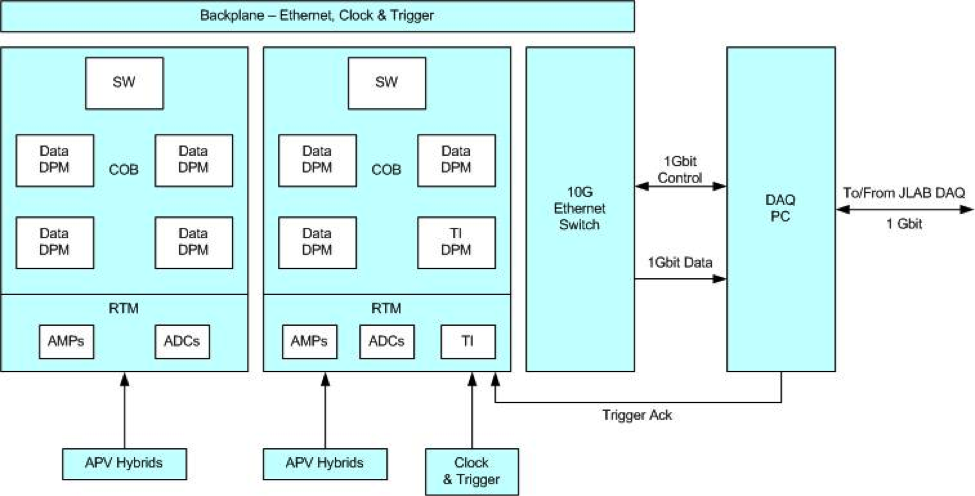
\includegraphics[scale=0.9]{test2012/daq/svt_daq_diagram.png}
\caption{\small{Schematic of the SVT DAQ used for the test run. Note that the hybrids are connected directly 
to the RTM and that an external DAQ PC is used for control and transfer of data to the JLab DAQ.}}
\label{fig:svtdaq}
\end{figure}
Being only half the size of the HPS SVT, the largest difference is the provision for
individual power and data for each sensor and readout chip from the power supplies and DAQ outside of the vacuum chamber.
This simplification reduced development time and cost at the expense of a large number of connections and vacuum feedthroughs.
With a total of 20 silicon microstrip sensors, each one connected to an onboard hybrid readout 
card hosting five 128-channel APV25 ASICs (shown in Figure ~\ref{fig:hybrid_and_apv25_testrun}), 600 lines for power and data are required.
 \begin{figure*}[t]
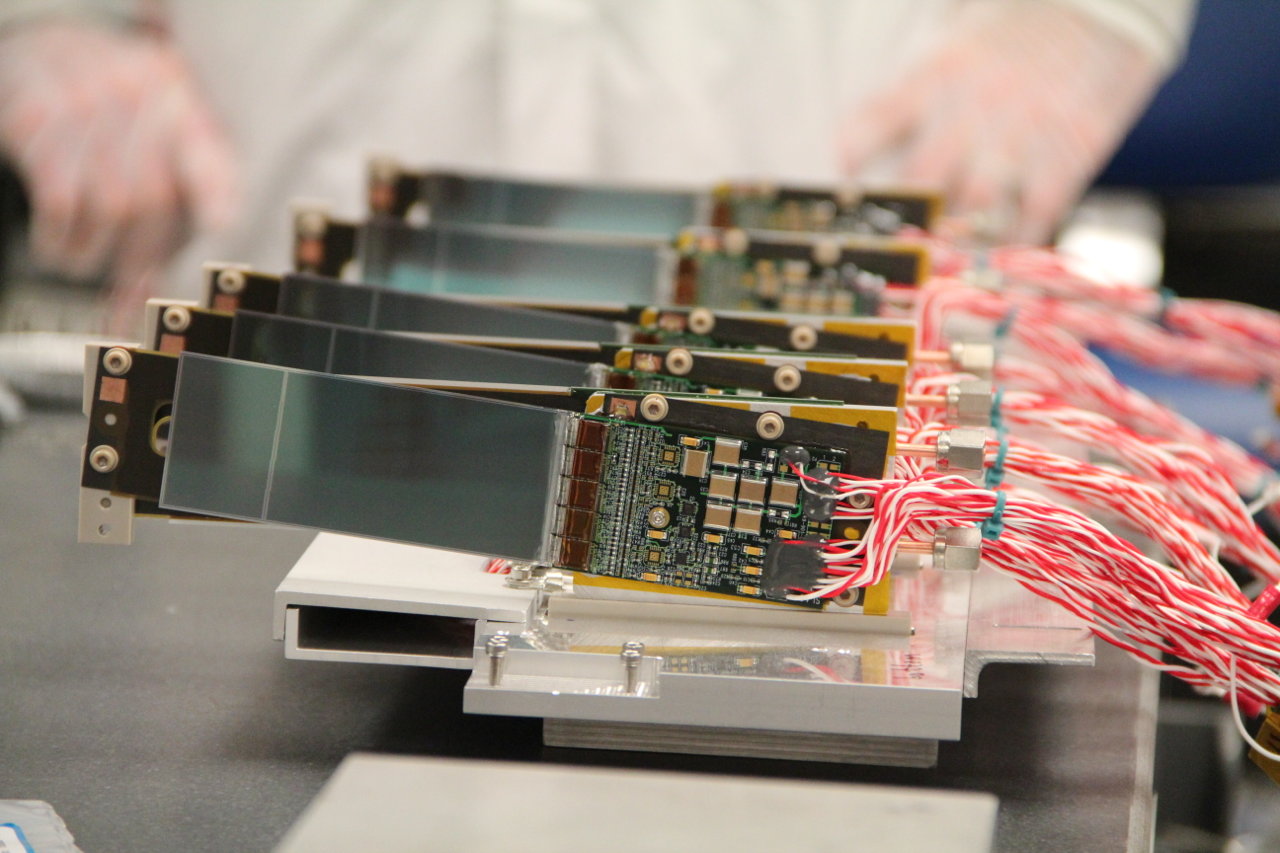
\includegraphics[ scale=0.3]{test2012/daq/svt_modules_on_sup_plate.png}
\caption{\small{View from upstream of one half of the SVT modules mounted on the support plate. Signal, 
power and control are soldered, and potted, to pads at one end while the five APV25 chips are wirebonded 
to the silicon sensor at the other.}}
\label{fig:hybrid_and_apv25_testrun}
\end{figure*}
Without optical conversion inside the chamber as proposed for HPS, analog signals from the APV25 chips are 
carried directly via multi-twisted-pair cable to ADCs on the Rear Transition Module (RTM), see Fig.~\ref{fig:rtm_testrun}, in the ATCA crate located outside the vacuum chamber. 
%The amplification and digitization is carried out on a Rear Transition Module (RTM) board designed specifically for the HPS test run. 
%On the RTM, a pre-amplifier converts the APV25 differential current output to a voltage output 
%scaled to the sensitive range of a 14-bit ADC. The RTM is organized into four sections with each section 
%supporting 3 hybrids (15 channels). The ADC is operated at the system clock of 41.667~MHz. 
%The RTM also includes a 4-channel Fiber Optic module and supporting logic which can be used to interface to the JLAB trigger supervisor card.
The ATCA main board, the Cluster on Board or COB (see Fig.~\ref{fig:rtm_testrun}), is similar to the one described for the HPS DAQ 
with the important exception that one of the Data Processing Modules (DPMs) functions as the trigger 
interface and there is no Reconfigurable Cluster Element (RCE) module. 
\begin{figure*}[t]
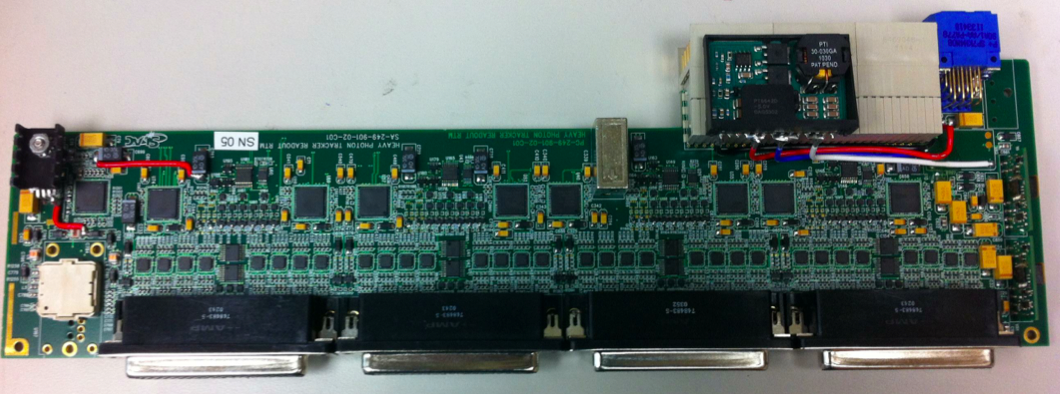
\includegraphics[ scale=0.25]{test2012/daq/rtm.png}
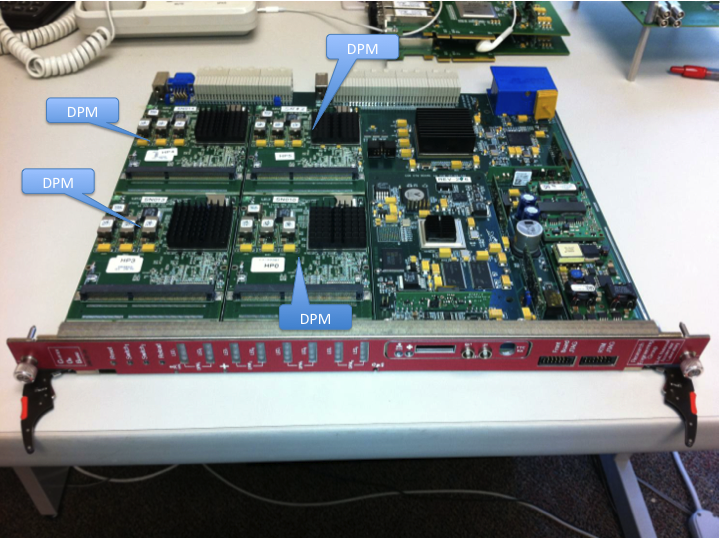
\includegraphics[ scale=0.4]{test2012/daq/svt_daq_module_noted.png}
\caption{\small{Picture of a RTM (top) and COB board (bottom) used in the HPS test run 2012.}}
\label{fig:rtm_testrun}
\end{figure*}
Instead, the DPMs package and send the data from the hybrids through a 1~Gbit ethernet connection to 
an external PC which serves the same purpose as the 
RCE module in the HPS DAQ. 
%The ATCA crate hosts two COB cards, one supporting four data processing DPMs and the other supporting three data processing DPMs and one trigger DPM for a total capacity of 21 hybrids, one more than required. 
The external PC also supports slow control and monitoring, communication with JLab DAQ, and trigger acknowledge interface to the trigger DPM in the ATCA crate. 
%to receive data from the ATCA crate. 
% , two standard 1~Gbit Ethernet and one custom low latency 
%data reception card. The first Ethernet interface is used for slow control and monitoring of the eight 
%DPM modules. The second Ethernet interface serves as the interface to the JLAB data acquisition system. The
%low latency network interface is used to receive data from the SVT ATCA crate and supports a low latency, 
%reliable, TTL trigger acknowledge interface to the trigger DPM. 
%This PC hosts the SVT control and monitoring 
%software as well as the ROC application described above.
